\section[Branching fraction of the decay \btophikmumu]
{Branching fraction of the decay $\boldsymbol{\btophikmumu}$}

The branching fraction of the signal decay \btophikmumu is determined relative to the normalization
channel \btojpsiphik:
\begin{equation}
  \BF\big(\btokphimumu\big)=
  \frac{ N^\prime\big(\btophikmumu\big) }{ N\big(\btojpsiphik\big) }
  \cdot\BF\big(\btojpsiphik\big)
  \cdot\BF\big(\jpsitomumu\big),
\end{equation}
here, $N^\prime\big(\btophikmumu\big)$ denotes the number of signal events extracted from an
weighted unbinned maximum likelihood fit of \btophikmumu candidates.
Each event is weighted by the relative efficiency:
\begin{equation}
  \frac{\varepsilon\big(\btojpsiphik\big)}{\varepsilon_{\qsq}\big(\btophikmumu\big)},
\end{equation}
where the denominator is the efficiency of the signal decay, \btophikmumu, in bins of \qsq.
The variation of efficiency in \qsq for the signal decay is shown in
\Fig{fig:hhh:effs}.
This is done because the efficiency of the decay \btophikmumu was shown to vary significantly over
the full \qsq range, the weights are determined in bins of \qsq.
The branching fraction measurements used were
$\BF\big(\btojpsiphik\big)=\big(5.2\pm1.7\big)\e{-5}$~\cite{PDG2012},
and $\BF\big(\jpsitomumu\big)=\big(5.93\pm0.06\big)\e{-2}$~\cite{PDG2012}.

Yields for both the signal and normalization channels are extracted from unbinned maximum
likelihood fits of the invariant mass of the \Bp candidates, these fits are shown in
\Fig{fig:phik:fit}.
The signal component for the normalization channel is the sum of two Gaussian functions, with a
power-law tail on the low mass side; the same function is used for fitting the weighted signal
distribution where all parameters are fixed from a fit to the high statistics normalization mode.
Combinatorial background is modelled as a second order Chebychev polynomial.
These fits give the values
$N^\prime\big(\btokphimumu\big)=25.2\,^{+6.0}_{-5.3}$ and
$N\big(\btojpsiphik\big)=1908\pm63$.
The statistical significance of this is $6.6\stdev$ according to Wilks' theorem~\cite{wilks1938}.

\begin{figure}
  \begin{center}
    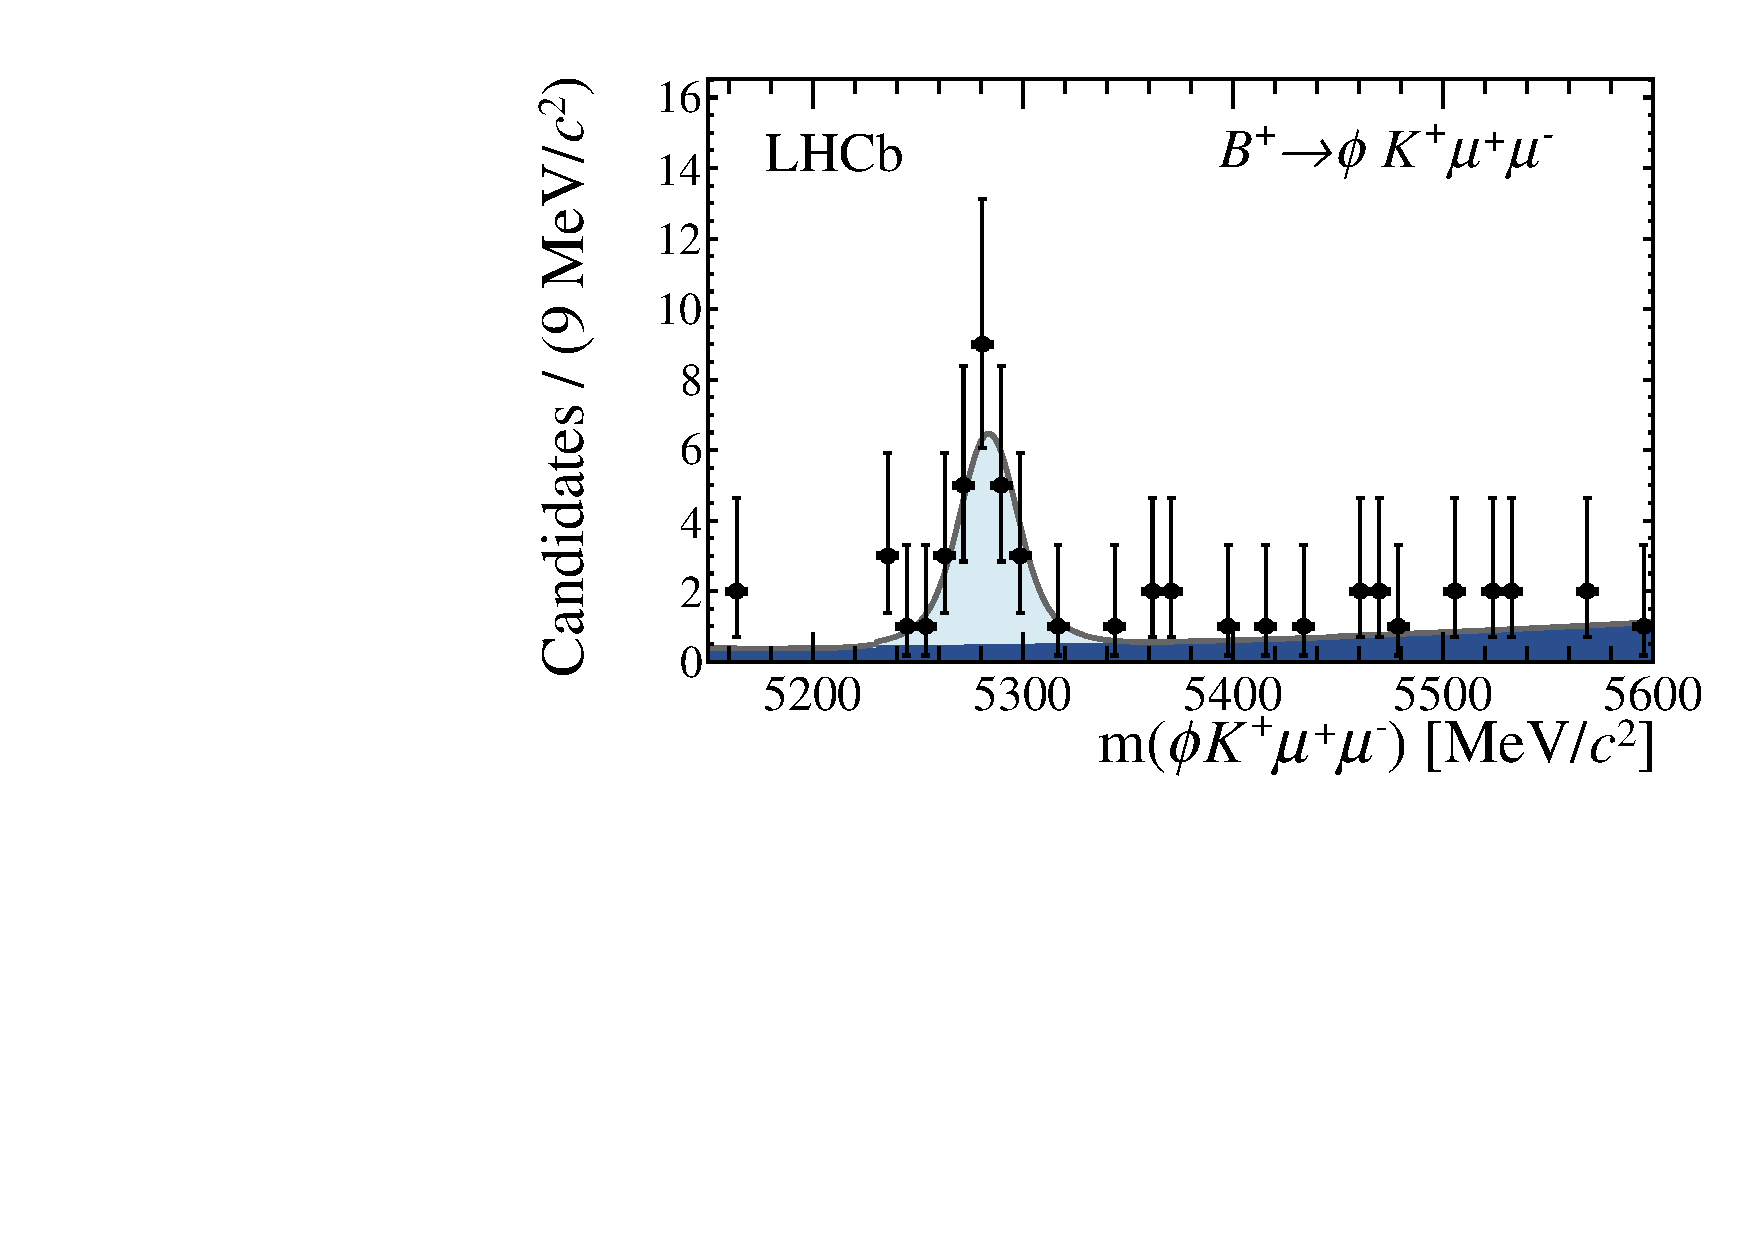
\includegraphics[width=0.48\textwidth]{b2phikmumu}
    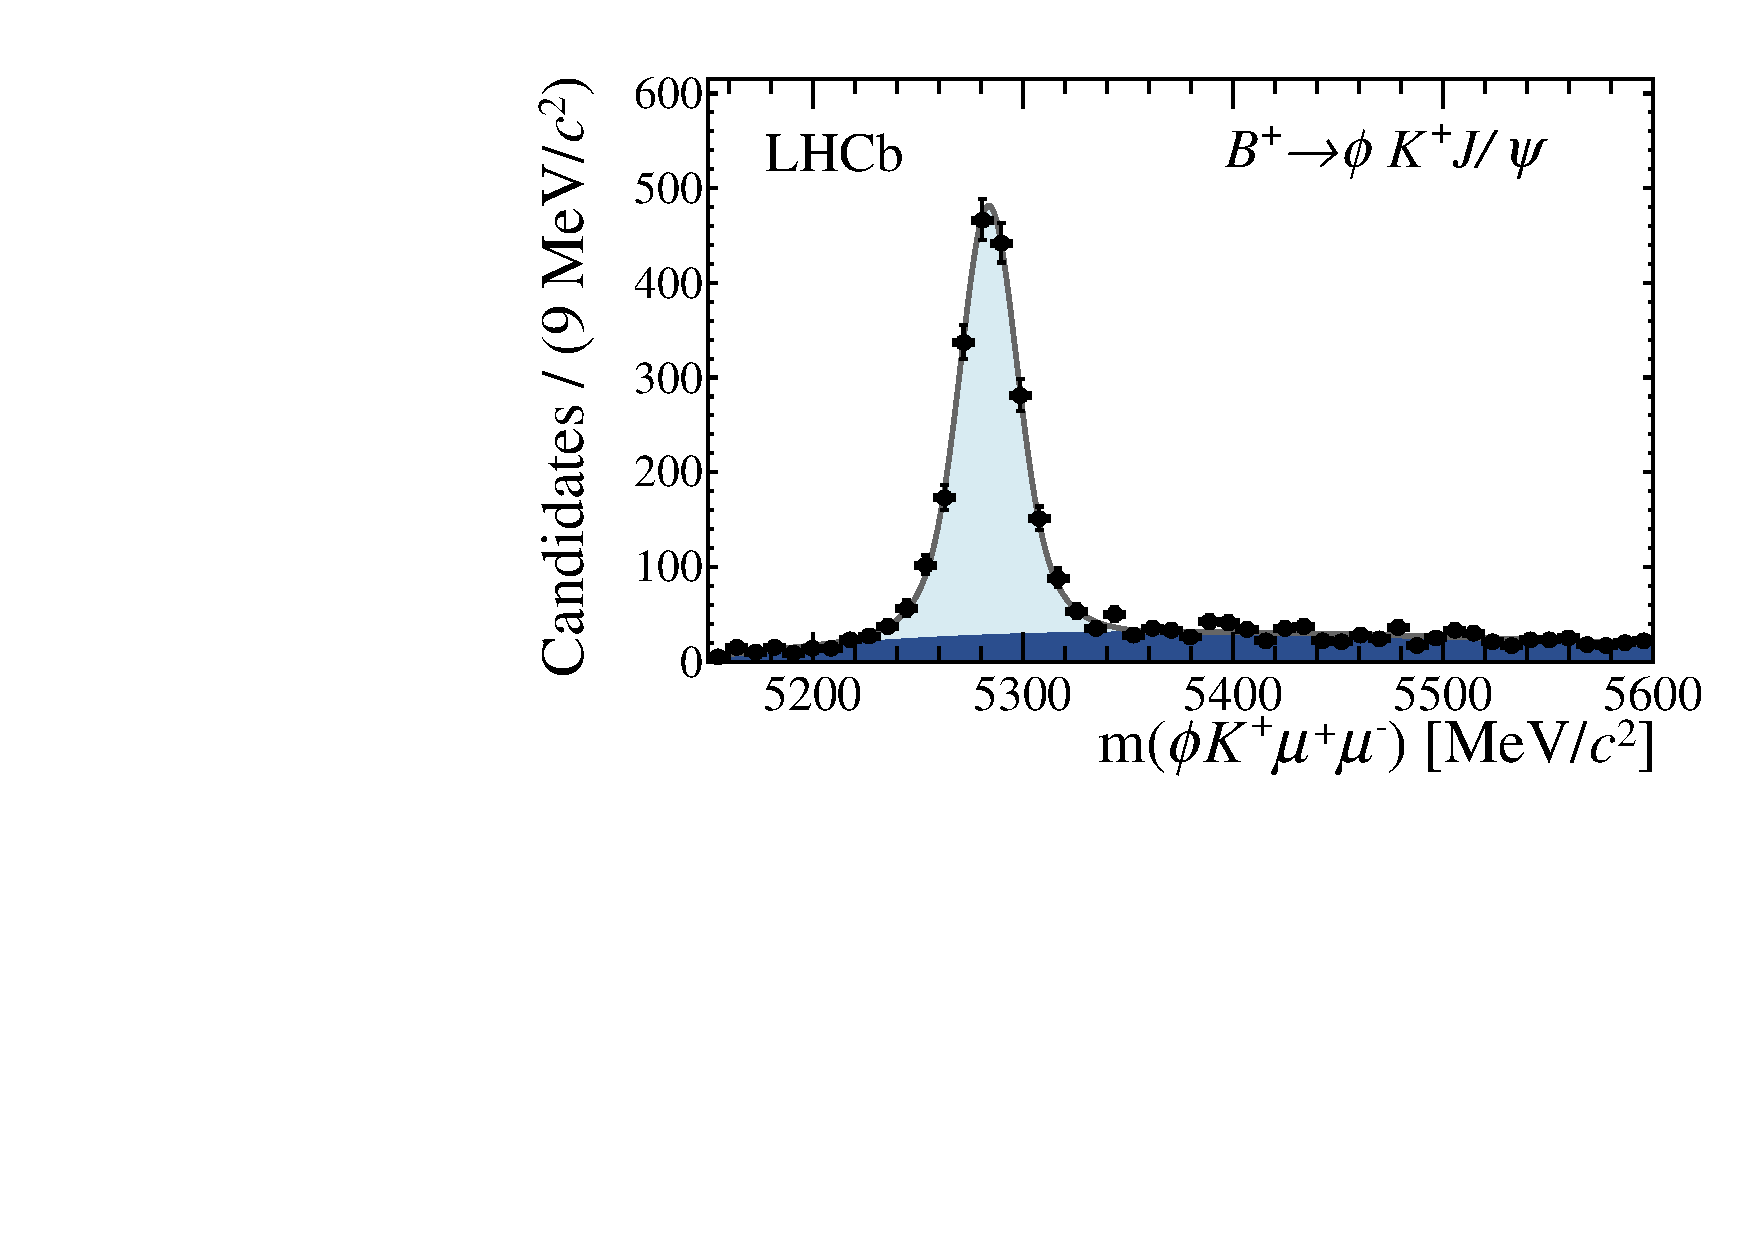
\includegraphics[width=0.48\textwidth]{b2phikjpsi}
    \caption[Fits to \btokphimumu and \btojpsiphik]
    {
      Invariant mass distributions for the
      (left) signal decay \btophikmumu, and
      (right) normalization mode \btojpsiphik.
      The signal component (light blue) is modelled by the sum of two Gaussian distributions, each
      with a power-law tail on the low-mass side; and the background component is a second order
      Chebychev polynomial.
      Variables describing the signal shape in the fit to \btophikmumu are fixed by the fit to
      \btojpsiphik.
    }
    \label{fig:phik:fit}
  \end{center}
\end{figure}

The above values lead to a measured branching fraction of
\begin{equation}
  \BF\big(\btophikmumu\big)=
  \big(0.81\,^{+0.18}_{-0.16}\stat\pm0.03\syst\pm0.27\normerr\big)\e{-7}.
\end{equation}
However, the charmonium vetoes remove $\big(2\,^{+10}_{-\pz2}\big)\pc$ of signal events, as
calculated using simulated events.
This systematic uncertainty in \btophikmumu is larger than in \btokpipimumu because the \qsq
distribution in the case of the former drops off and ends in the \jpsi region, as shown in
\Fig{fig:phik:q2}.
Taking this into account results in a value of
\begin{equation}
  \BF\big(\btophikmumu\big)=
  \big(0.82\,^{+0.19}_{-0.17}\stat\,^{+0.10}_{-0.04}\syst\pm0.27\normerr\big)\e{-7}.
\end{equation}
The ratio of branching fractions of the signal and normalization channels is
\begin{equation}
  \frac{ \BF\big(\btophikmumu\big) }{ \BF\big(\btojpsiphik\big) }
  =\big(1.58\,^{+0.36}_{-0.32}\stat\,^{+0.19}_{-0.07}\syst\big)\e{-3},
\end{equation}
which is quoted because there are large relative uncertainties associated with the branching
fraction of the normalization channel (\approx$1\,\%$).

\begin{figure}
  \begin{center}
    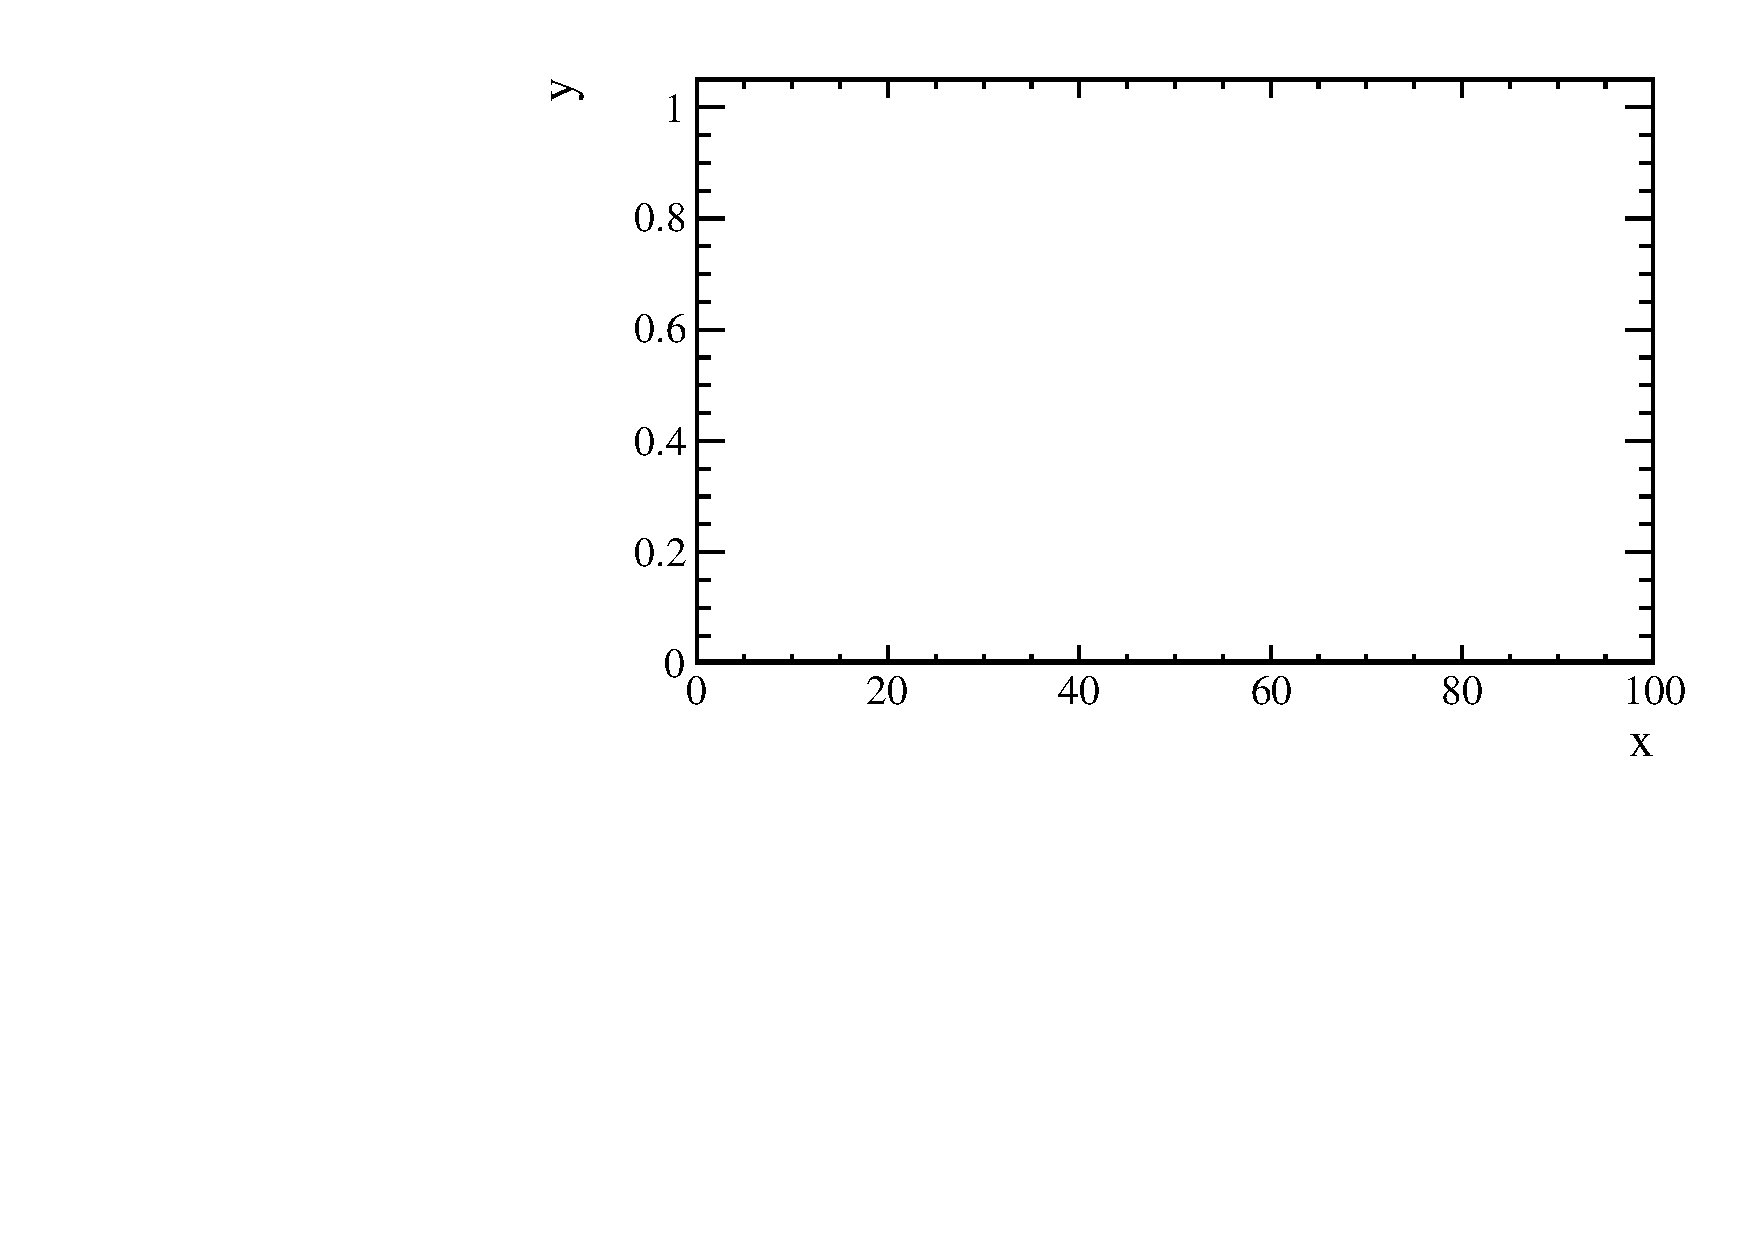
\includegraphics[width=0.48\textwidth]{blank}
    \caption[CHIPS]
    {
      \qsq shape of \phik.
    }
    \label{}
  \end{center}
\end{figure}


Just as in \kpipi, it is expected that the \phik system will be composed of numerous strange
resonances.
However, low statistics and some phasespace limitations make it impossible to draw and meaningful
conclusions.
The background subtracted \phik distributions for the signal and normalization channels are shown
in \Fig{fig:phik:phik}.
\bam{MORE HERE.}


\begin{figure}
  \begin{center}
    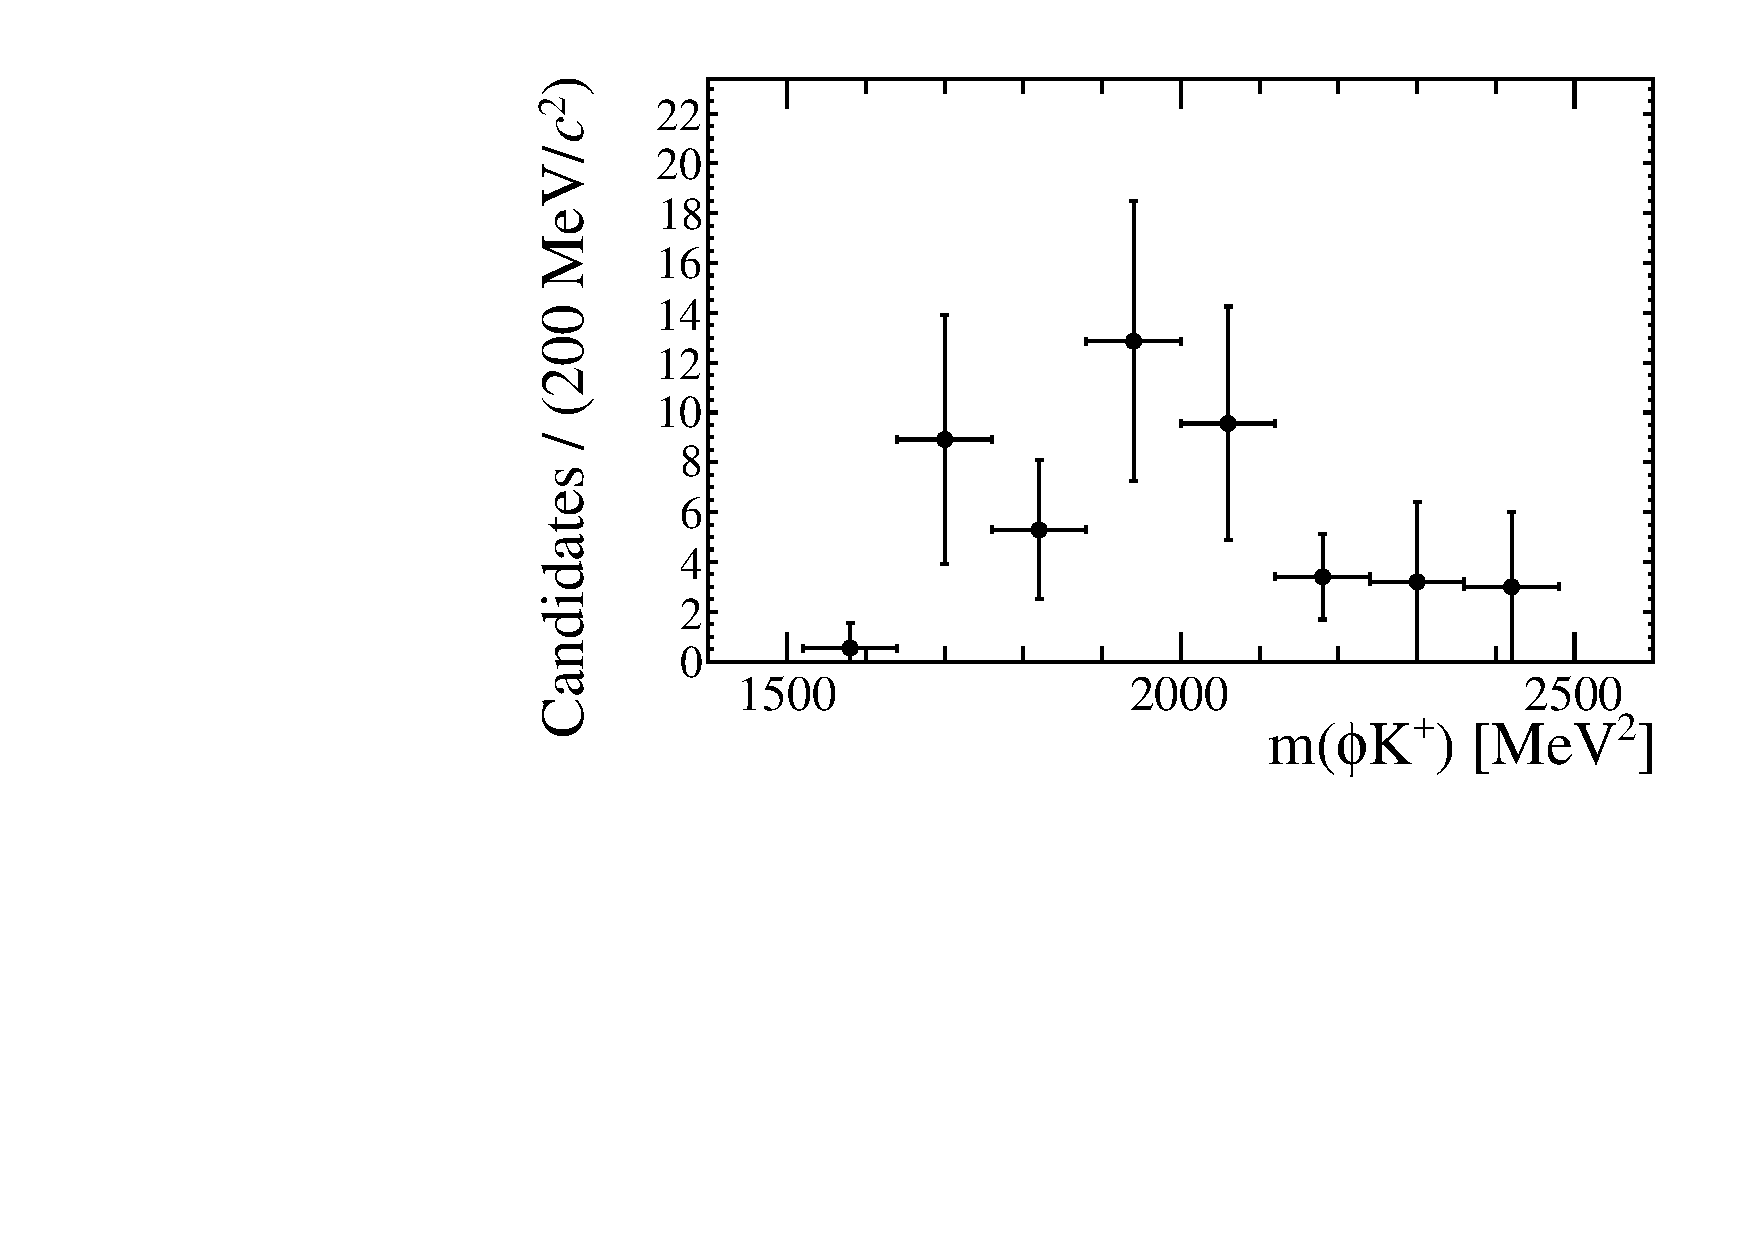
\includegraphics[width=0.48\textwidth]{phik_frommumu}
    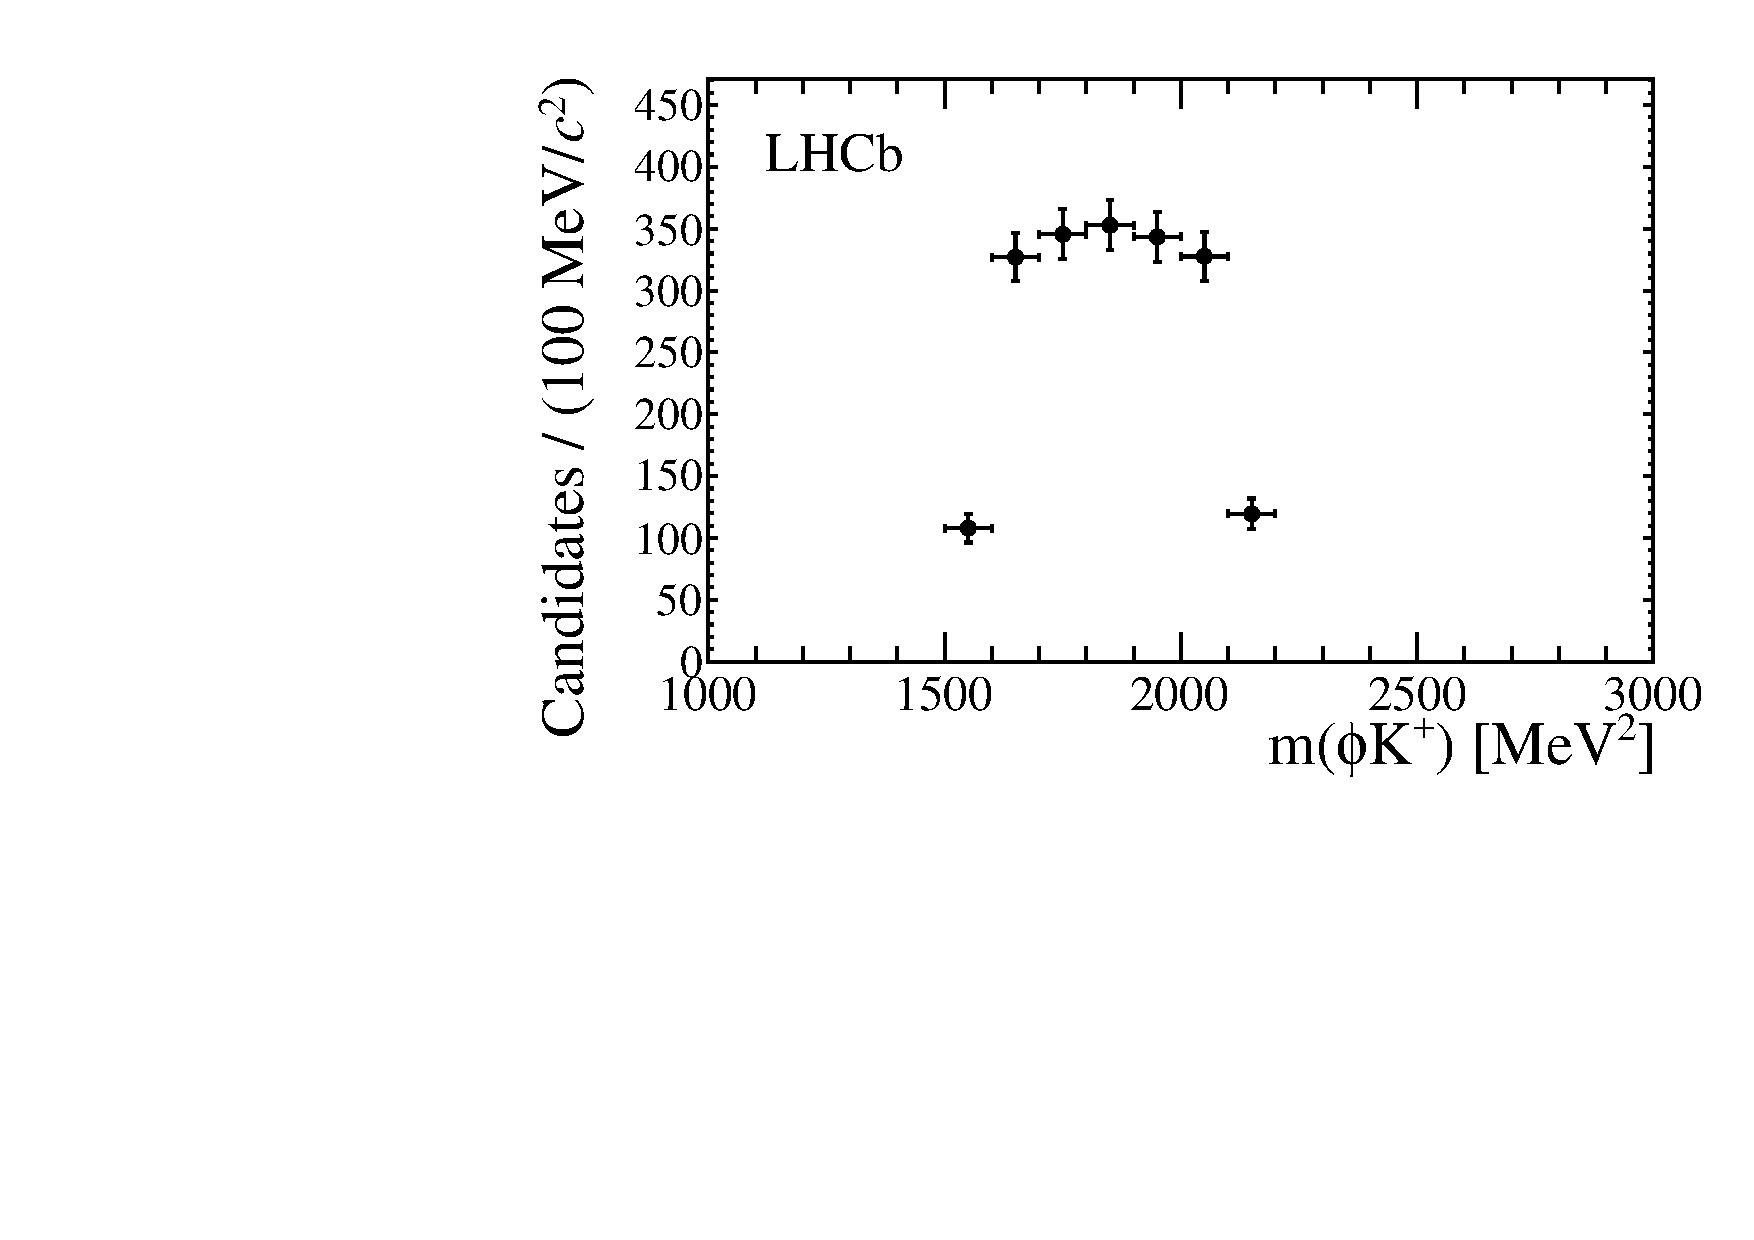
\includegraphics[width=0.48\textwidth]{phik_fromjpsi}
    \caption[Invariant mass distributions of \phik]
    {
      Distributions of the sWeighted invariant mass \phik object from the decay
      (left) \btophikmumu, and
      (right) \btojpsiphik.
    }
    \label{fig:phik:phik}
  \end{center}
\end{figure}




%The normalization channel has a large relative uncertaity on its measured branching fraction
%$\BF\big(\btojpsiphik\big)=\big(5.2\pm1.7\big)\e{-5}$~\cite{PDG2012}.
%With


\subsection{Systematic uncertainties}
\label{ssec:phik:syst}

Systematic uncertainties contributing to the measurement of $\BF(\btophikmumu)$ are determined in
very similar ways as for the measurement of $\BF(\btokpipimumu)$, as detailed in
\Sec{ssec:kpipi:syst}.
The uncertainties introduced by correcting the simulated events by weighting and resampling are
calculated in the same way as for the decay \btokpipimumu.
The systematic uncertainty arising from the signal mass model was evaluated by
substituting the nominal double Gaussian with a power-law tail, for a single Gaussian with a tail
and recalculating the signal yield.
Similarly, the systematic from the background model is evaluated by repeating the fit with a first
order, rather than a second order, polynomial.
These changes in the fit model lead to to a total systematic uncertainty of \approx$3\pc$.
The uncertainty on the \qsq distribution in the simulation was estimated by reweighting the from
the nominal phasespace simulation to the distribution of the \decay{\Bp}{\kone{1270}\mumu} mode.
Therefore, a photon pole at low \qsq is introduced.
The total systematic uncertainty evaluates to \approx$1.5\pc$.

The fraction of events that are removed by the charmonium vetoes are determined from simulation.
But, as discussed, the \qsq distribution that is described by the \btophikmumu simulation was
inaccurate since there is no theoretical prediction available.
To circumnavigate this problem, generator level simulated events is used to obtain the central
value.
Vetoed fractions are then calculated by generating events whose \qsq distribution is taken from the
\decay{\Bp}{\kone{1270}\mumu} decay, where the mass of the \kone{1270} system is replaced with an
estimated mass of the \phik system.
The value of $m_{\phik}=1960\mev$, which is taken fro the sWeighted $m_{\kpipi}$ distribution from
data.
In this way, it was determined that $(2\,^{+10}_{-\pz2})\,\%$ of signal events were removed by the
charmonium vetoes.

All other systematic uncertainties are evaluated in the same way as in the analysis of the decay
\btokpipimumu, and are summarized in \Table{tab:phik:syst}.


\begin{table}
  \caption[Systematic uncertainties on the branching fraction of \btophikmumu]
  {
    Systematic uncertainties on the branching fraction of \btophikmumu.
  }
  \label{tab:phik:syst}
  \begin{center}
  \begin{tabular}{lc}\toprule
    Source & $[\times10^{-8}]$
    \\\midrule
    $\BF\big(\btojpsiphik\big)$  &   2.688        \\  % x10e-8
    %%\littlerule
    %Tracking efficiency          &   0.057        \\  % x10e-8
    %Reweighting                  &   0.020        \\  % x10e-8
    %PID resampling               &   0.047        \\  % x10e-8
    %Muon PID efficiencies        &   0.013     \\  % x10e-8
    %Relative efficiency          &   0.065        \\  % x10e-8
    %Background mass model        &   0.245        \\  % x10e-8
    %Signal mass model            &   0.128        \\  % x10e-8
    %Trigger                      &   0.123        \\  % x10e-8
    %\qsq model                   &   0.118        \\  % x10e-8
    %%\littlerule
    %%Charmonium veto        &   $^{+0.931}_{-0.166}$ \\
    Corrections to simulation    &   0.145 \\
    Relative efficiency          &   0.065 \\
    Mass model: background       &   0.245 \\
    Mass model: signal           &   0.128 \\
    \qsq model                   &   0.118 \\
    %\littlerule
    %Charmonium veto        &   $^{+0.931}_{-0.166}$ \\
    \bottomrule
  \end{tabular}
\end{center}
\end{table}


%To circumnavigate this dilemma


%reweighting etc same as above...
%signal, single, not nominal double CB
%bkg, linear, not second order
%qsq by reweighting to nominal phasespace dist for B to K1(1270).
%
%circumvanvigate this dilemma
%
%Charmonium vetoes,
%vetoed fractions





